\renewcommand{\labelenumi}{\arabic{enumi}.}

\section{Formulário de avaliação SustenAgro\label{sec:Formul=0000E1rio-de-avalia=0000E7=0000E3o-SustenAgro}}

O processo consiste em realizar cinco tarefas descritas a continuação,
e responder as seguintes três perguntas para cada tarefa: 
\begin{itemize}
\item Conseguiu realizar a tarefa?
\item Teve algum problema/dúvida durante a realização da tarefa?
\item Tem sugestões que permitam melhorar/facilitar a realização da tarefa?
\end{itemize}

\subsection*{Tarefa 1}

Cadastrar usuário:
\begin{enumerate}
\item Ingressar no software SustenAgro em http://java.icmc.usp.br:1300/
\item Dar click na opção de 'Inscrever-se' e ingressar no formulário de
cadastro de novo usuário
\item Preencher o formulário e enviar
\item Ingressar ao sistema com seus dados cadastrados. 
\end{enumerate}

\subsection*{Tarefa 2}

Cadastrar uma unidade produtiva: 
\begin{enumerate}
\item Dar click no link de 'Avaliação'
\item Cadastrar no formulário de uma nova unidade produtiva.
\item Preencher o formulário e enviar 
\end{enumerate}

\subsection*{Tarefa 3}

Preencher dados da avaliação: 

Se a anterior tarefa foi realizada com sucesso, o sistema vai encaminhá-lo
ao formulário de nova avaliação, em caso negativo pode dar click no
botão 'Análises' e 'Nova Análise', para realizar:
\begin{enumerate}
\item Preencher alguns dados de avaliação de eficiência e custo
\item Preencher alguns dados de avaliação da sustentabilidade
\item Solicitar avaliação por meio do botão 'Avaliar' 
\end{enumerate}

\subsection*{Tarefa 4}

Visualizar os resultados: 

Se a anterior tarefa foi realizada com sucesso, o sistema vai encaminhá-lo
a tela de 'Resultados da avaliação', em caso negativo pode dar click
no botão 'Análises' e selecionar a análise cadastrada, para realizar:
\begin{enumerate}
\item Visualizar a planilha de eficiência e custo
\item Visualizar a planilha de sustentabilidade
\item Visualizar o relatório da avaliação
\item Visualizar os dados da avaliação na aba 'Avaliação'
\end{enumerate}

\subsection*{Tarefa 5}

Editar avaliação: 
\begin{enumerate}
\item Na tela de 'Resultados da avaliação' selecionar a aba 'Avaliação'
\item Acrescentar alguns dados de avaliação de eficiência e custo
\item Acrescentar alguns dados de avaliação da sustentabilidade
\item Solicitar a atualização por meio do botão 'Atualizar' 
\end{enumerate}

\section{Formulário de avaliação Decisioner\label{sec:Formul=0000E1rio-de-avalia=0000E7=0000E3o-Decisioner}}

O processo consiste em realizar cinco tarefas descritas a seguir,
e responder as seguintes três perguntas para cada tarefa:
\begin{itemize}
\item Conseguiu realizar a tarefa?
\item Teve algum problema/dúvida durante a realização da tarefa?
\item Tem sugestões para melhorar/facilitar a realização da tarefa?
\end{itemize}
As seguintes tarefas devem ser realizadas na interface de administração
do sistema:

\subsection*{Tarefa 1}

Cadastrar novo indicador
\begin{enumerate}
\item Ingressar com login de administrador no software SustenAgro em http://java.icmc.usp.br:1300/
\item Dar click no link 'Ontology'
\item Clicar em Feature, Indicador, Indicador de Sustentabilidade e Dimensão
Social
\end{enumerate}
Cadastrar uma nova dimensão, atributo e indicador a partir da linha
1020 no seguinte formato:

\begin{algorithm}[h]
\inputencoding{latin9}\begin{lstlisting}[caption={C�digo de novo indicador}]
AgriculturalIndicator: 
 is_a: SustainabilityIndicator 
 relevance: 1.0 
 label: 
  - Agricultural dimension @en 
  - Dimens�o agricultural @pt

DeforestationAttribute: 
 is_a: AgriculturalIndicator 
 label: 
  - Atributo desmatamento @pt 
  - Deforestation attribute @en 

DeforestationIndicator: 
 is_a: DeforestationAttribute 
 label: 
  - Indicador desmatamento @pt 
  - Deforestation indicator @en 
 relevance: 2.0 
 value: YesNo
\end{lstlisting}
\inputencoding{utf8}\end{algorithm}

\begin{enumerate}
\item Dar click na opção “Save”
\item Acrescentar a nova dimensão na DSL, clicando na Aba DSL e no link
Main adicionar na linha 106 o seguinte código
\item \inputencoding{latin9}
\begin{lstlisting}[caption={Adi��o de feature na DSL}]
feature ':AgriculturalIndicator'
\end{lstlisting}
\inputencoding{utf8}\item Dar click na opção “Save” - Procurar o indicador cadastrado na interface
de Usuário, na tela de Usuário na aba Avaliação selecionar uma Unidade
Produtiva e ir em Nova Avaliação
\end{enumerate}

\subsection*{Tarefa 2}

Editar a fórmula de avaliação 
\begin{enumerate}
\item Dar click no link 'DSL'
\item Procurar o comando Report e editar algum valor da fórmula
\item Dar click na opção “Save”
\item Visualizar os índices de uma avaliação cadastrada no sistema por meio
da aba Report, na tela de Usuário na aba Avaliação selecionar uma
Unidade Produtiva, selecionar uma Avaliação e um Report ligado a ela.
\end{enumerate}

\subsection*{Tarefa 3}

Editar os limiares das widgets matriz e semáforo de avaliação
\begin{enumerate}
\item Dar click no link 'DSL'
\item Procurar o comando sustainabilityMatrix e editar o valor de range\_x
\item Procurar o comando sustainabilitySemaphore e editar o valor de range
\item Dar click na opção “Save”
\item Visualizar os índices de uma avaliação cadastrada no sistema, na tela
de Usuário na aba Avaliação selecionar uma Unidade Produtiva, selecionar
uma Avaliação e um Report ligado a ela
\end{enumerate}

\subsection*{Tarefa 4}

Editar uma View
\begin{enumerate}
\item Dar click no link 'Views'
\item Selecionar uma a view de contact
\item Editar o título da view por meio do comando pageHeader
\item Dar click na opção “Save”
\item Visualizar a view na interface do Usuário por meio do link Contact
\end{enumerate}

\subsection*{Tarefa 5}

Editar labels das internationalizations
\begin{enumerate}
\item Dar click no link 'Internationalization'
\item Seleccionar ingles
\item Editar o texto de um label
\item Dar click na opção “Save”
\item Visualizar uma view que faça uso do label editado na interface do
Usuário
\end{enumerate}

\section{Formulário Delphi para Workshop SustenAgro\label{sec:Formulario-Delphi-Workshop}}

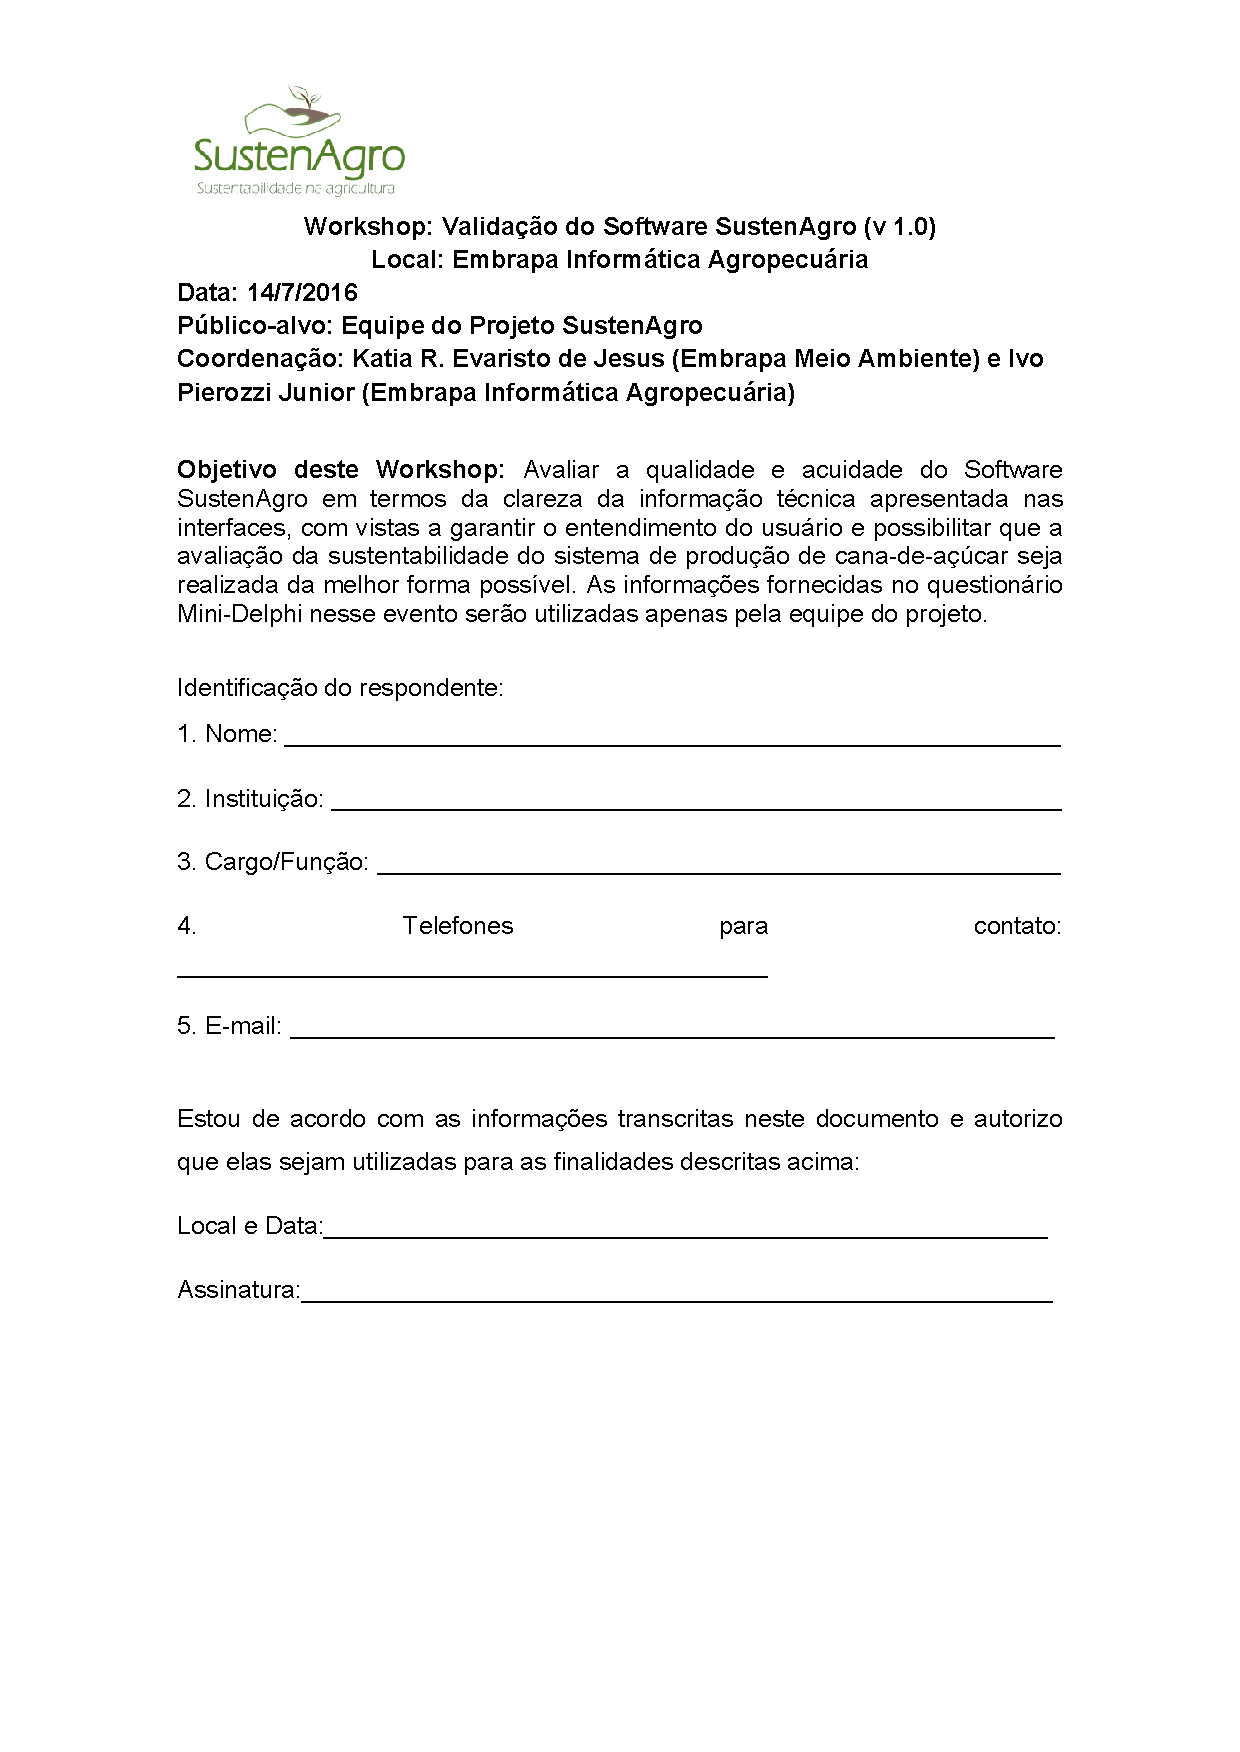
\includepdf[pages=-,width=1\paperwidth]{pages/workshop}
